Das Cox-Ross-Rubinstein-Modell (kurz: CRR-Modell) wird auch Binomialmodell genannt und wurde 1979 von Cox, Ross und Rubinstein entwickelt.

Es handelt sich dabei um ein Modell für die Preisentwicklung eines Wertpapiers plus ein Verrechnungskonto mit konstanter Verzinsung (Numeraire) in diskreter Zeit.

\textbf{Parameter:}

\begin{center}
	\begin{tabular}{|c|l|}
		\hline
		$r$ & Zinsrate \\ \hline
		$b$ & Rendite des Wertpapiers bei Aufwärtsbewegung (''up``) \\ \hline
		$a$ & Rendite des Wertpapiers bei Abwärtsbewegung(''down``) \\ \hline
		$p \in (0,1)$ & Wahrscheinlichkeit für ''up`` \\ \hline
		$S_0 > 0$ & Preis Wertpapier zum Zeitpunkt Null \\ \hline
		$N \in \N$ & Anzahl der Zeitschritte \\ \hline
	\end{tabular}
\end{center}

\textbf{Annahmen:} $r > -1$, $b > a > -1$

Wir modellieren Wertpapiere $\folge{S_k}{k \in [N]}$ und Verrechnungskonto $\folge{S_k^0}{k \in \N}$ als stochastische Prozesse auf einem Wahrscheinlichkeitsraum $(\Omega, \F, \P)$.

\begin{itemize}
	\item $S_0^0 = 1$ und $S_n^0 = (1+r)^n$
	\item Wir definieren die \begriff{Rendite} $R_n(\omega)$ in der $n$-ten Marktperiode durch
	\begin{equation*}
		R_n = \begin{cases} b & \mit p \\ a & \mit 1-p \end{cases}
	\end{equation*}
	Die Renditen $(R_1, \dots, R_N)$ sind unabhängig.
	\begin{equation*}
		S_n = S_0 * \prod_{k=1}^n (1+R_k)
	\end{equation*}
	
	Der Verlauf von $S$ lässt sich grafisch als Binomialbaum darstellen:
	
	\begin{center}
		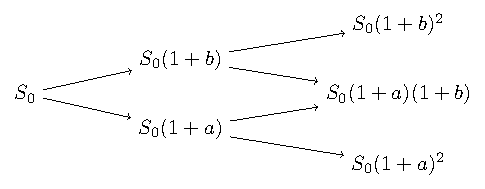
\includegraphics[width=.5\textwidth]{stochv_abbildungen/stochv_1_2_crr.pdf}
	\end{center}
	
	Man nennt dies auch ein ''rekombinierendes Baummmodell``. Es hat den Vorteil, dass die Anzahl der Knoten nur linear mit $n$ wächst.
	
	\item Abgezinster Preisprozess $\schlange{S}_n \defeq \frac{S_n}{S_n^0} = S_0 * \prod_{k=1}^n \frac{1+R_k}{1+r}$.
	
	\item Filtration: natürliche Filtration $\F_n = \sigma \brackets{S_1, \dots, S_n}$.
\end{itemize}

\begin{proposition} %2.1
	Im CRR-Modell gilt:
	\begin{enumerate}[label=(\alph*)]
		\item Die Anzahl der Aufwärtsbewegungen $U_n \defeq \# \menge{k \in [n] \colon R_k = b}$ ist binomialverteilt, d.h. $U_n \sim \Bin(n,p)$.
		\item Es gilt 
		\begin{equation*}
			\log\brackets{\frac{\schlange{S}_n}{S_0}} = U_n \log\brackets{\frac{1+b}{1+a}} + n \log\brackets{\frac{1+a}{1+r}}
		\end{equation*}
		d.h. $\log\brackets{\frac{\schlange{S}_n}{S_0}}$ ist nach Skalen-Lagen-Transformation binomialverteilt.
		\item Die Verteilung von $S_n$ ist gegeben durch
		\begin{equation*}
			\P\brackets{S_n = S_0 (1+b)^k (1+a)^{n-k}} = \binom{n}{k} p^k (1-p)^{n-k}
		\end{equation*} 
	\end{enumerate}
\end{proposition}

\begin{proof}
	\begin{enumerate}[label=(zu \alph*), leftmargin=\zulength]
		\item klar
		\item $\frac{\schlange{S}_n}{S_0} = \brackets{\frac{1+b}{1+a}}^{U_n} * \brackets{\frac{1+a}{1+r}}^n \follows \log\brackets{\frac{\schlange{S}_n}{S_0}} = U_n \log\brackets{\frac{1+b}{1+a}} + n \log\brackets{\frac{1+a}{1+r}}$
		\item Es ist $S_n = S_0 (1+b)^{U_1}(1+a)^{n-U_n} $. Also
		\begin{equation*}
			\P\brackets{S_n = S_0 (1+b)^k (1+a)^{n-k}} = \P(U_n = k) \overset{(a)}{=} \binom{n}{k} p^k (1-p)^{n-k}
		\end{equation*}
	\end{enumerate}
\end{proof}

\begin{*bemerkung_inline}
	Teil (b) suggeriert Konvergenz von $\log\brackets{\frac{\schlange{S}_n}{S_0}}$ gegen Normalverteilung für $n \to \infty$ (nach Skalierung) 
	$\leadsto$ Black-Scholes-Modell ($\nearrow$ Kapitel 3).
\end{*bemerkung_inline}